\documentclass[a4paper,conference]{IEEEtran}

	\ifCLASSINFOpdf
	\usepackage{graphicx}
	  \DeclareGraphicsExtensions{.pdf,.jpeg,.png,.eps,.jpg}
	\else
	\fi
	\usepackage{booktabs}
	\usepackage{tabularx}
	\usepackage{multirow}
	\usepackage{amsmath}
	\usepackage{url}
	\usepackage{hyperref}
		\hypersetup{
			colorlinks,
			citecolor=black,
			filecolor=black,
			linkcolor=black,
			urlcolor=blue
		}

		\graphicspath{{assets/}}
	
	\begin{document}
	
	\title{Image Classifier using Tensorflow on ARMv7 Architecture}
	
	\author{\IEEEauthorblockN{Akshit Bhalla}
	\IEEEauthorblockA{Department of Electronics and Communication Engineering\\
	B.M.S. College of Engineering\\Bangalore, India\\\url{https://akshitbhalla.co}}
	\and
	\IEEEauthorblockN{Dr. Suma M N}
	\IEEEauthorblockA{Associate Professor, \href{mailto:suma.ece@bmsce.ac.in}{suma.ece@bmsce.ac.in}\\Department of Electronics and Communication Engineering\\
	B.M.S. College of Engineering\\Bangalore, India}
	}
	
	
	\maketitle
	
	\begin{abstract}
	
	Image Recognition of objects in the real world is required to enable correct and safe interactions for specially-abled people (those affected by a deficiency of sight) with their environment. For identification, a general-purpose image classifier has been created that is of high efficiency to allow it to work on embedded devices (wearables) and of high accuracy for the large number of real world items that it has been trained to identify (over 1000 categories). A low-cost ARM microcontroller and camera are the minimum requirements to be able to execute this classifier. Further enhancements have been demonstrated in the forms of Text-To-Speech implementation and external display attachment to indicate possible object probabilities in this project.
	
	\end{abstract} 
	
	\section{Introduction} \label{Introduction}
	 
	Our brain consists of 86 billion interconnected neurons. Each neuron responds to certain stimuli and passes output to another. For example, there may be some dedicated to recognizing trees (some for the roots, bark, branches and leaves), each having a different weighting (based on how important that feature is) to the overall contribution. If all of them activate correctly, our brain tells us that we saw a tree. In Machine Learning, artificial neural networks (modeled on the brain) are used to calculate probabilities for features that they are trained to identify.

	In order to help the specially-abled who do not have a normal sense of sight, a device aimed at utilising Image Processing techniques on embedded platforms has been created in order to help them identify the objects around them and enable them to interact with the world more easily and safely. 

	The hardware board chosen for this project is the Pico i.MX7D, which implements the ARM Cortex-A7 core as well as the ARM Cortex-M4 core. The dual-core
architecture enables the device to run a rich operating system like Linux on the Cortex-A7 core and an RTOS
on the Cortex-M4 core.\\
\newline
The ARM Cortex-M4 and Cortex-A7 range of microcontroller cores are high performance and
low power 32-bit RISC processors.
	
	\begin{itemize}
		\item Dual ARM Cortex-A7 which operates at speeds of up to 1.2 GHz.
		\item Cortex-M4 up to 200 MHz.
		\item 512 KB L2 cache.
		\item Gigabit Ethernet
		\end{itemize}
		
	\section{Literature Survey} \label{section:literature_survey}
	


	\subsection{Cortex-A7} \label{subsection:Cortex-A7}

	The Application-A profile defines an architecture aimed at high performance
	processors, supporting a virtual memory system using a Memory Management
	Unit (MMU) and therefore capable of running fully featured operating systems.
	Support for the ARM and Thumb instruction sets is provided
	
	\begin{itemize}
		\item Modified Harvard Architecture (separate, concurrent access to instructions and data).
		\item Load/Store Architecture.
		\item Thumb-2 technology as standard. This is discussed below at \ref{subsection:Thumb}
		\item Less than \(0.5mm^2\), using \(28nm\) process technology.
		\item Floating Point Unit (FPU)
	  \end{itemize}

	  \subsection{Cortex-M4} \label{subsection:Cortex-M4}

The Microcontroller-M profile defines an architecture aimed at low cost systems,
where low-latency interrupt processing is vital. Cortex-M processors differ from other processors in
ARM’s range in that they execute only Thumb-2 instructions and do not support the complete ARM
instruction set.

\begin{itemize}
    \item Efficient Harvard architecture 3-stage pipeline core (Fetch-Decode-Execute). 
    \item 32-bit processor, including 32-bit address and data buses.
    \item 4GB address space and up to 2GB for RAM (either on or off chip).
    \item A Nested Vectored Interrupt Controller (NVIC) for low-latency interrupt processing.
    \item Memory Protection Unit (MPU).
    \item Fixed Memory Map for easy porting of software between systems based on Cortex-M4.
  \end{itemize}

  \subsection{Thumb Instruction Set} \label{subsection:Thumb}

Thumb instructions are each 16 bits long, and have a corresponding 32-bit ARM instruction that has the same effect. The main reason for using Thumb code is to reduce code density. Because of its
improved density, Thumb code tends to cache better than the equivalent ARM code and can
reduce the amount of memory required. The complete ARM instruction set may be used for particular code sections which require the highest performance.

\subsection{Image Processing} \label{subsection:image_processing}
	
Image processing is a method to convert an image into digital form and perform some operations on it to extract some useful information from it. It is a type of signal dispensation in which the input is an image and the output is the characteristics associated with that image. The system includes treating images as two dimensional signals while applying already set signal processing methods to them. 

Image processing includes these steps:

\begin{itemize}
\item Importing the image from either the storage device or by digital photography using a camera.
\item Analysing and manipulating the image. This includes compression and image enhancement in order to find predictable patterns in the data.
\item A probability report on object identification based on the image data.
\end{itemize}


The purpose of image processing may be broadly classified by the following:

\begin{enumerate}
\item Visualization - Identify areas in the image that are of interest.
\item Image Sharpening and Restoration - To create a more workable dataset.
\item Identification of Patterns - Applying the image classifier on available data.
\item Image Recognition - Distinguish between the objects found in an image.

\end{enumerate}

	\section{Methodology and Implementation} \label{section:methodology}
	
	\subsection{Classifier} \label{subsection:classifier}

	A Single-Shot-Detection (SSD) image classifier is used. Prior detection systems repurpose classifiers or localizers to perform detection. They apply the model to an image at multiple locations and scales. High scoring regions of the image are considered detections. \\We apply a single neural network to the full image. This network divides the image into regions and predicts bounding boxes and probabilities for each region. These bounding boxes are weighted by the predicted probabilities.\\
	\newline
	This model has several advantages over classifier-based systems. It looks at the whole image at test time so its predictions are informed by global context in the image. It also makes predictions with a single network evaluation unlike systems like R-CNN which require thousands for a single image. This makes it extremely fast, more than 1000x faster than R-CNN and 100x faster than Fast R-CNN.\\
	\newline
	It uses the TensorFlow Lite inference library and does not require any native build tools. \\
	\newline
	
	\subsection{Hardware Model} \label{subsection:hardware}

	When a button is pushed or when the touhscreen is touched, the current image is captured from the camera. The image is then converted and piped into a TensorFlow Lite classifier model that identifies what is in the image. Up to three results with the highest confidence returned by the classifier are shown on the screen, if there is an attached display. Also, the result is spoken out loud using Text-To-Speech to the default audio output.

	\begin{figure}[h] 
		\centering
		\resizebox{8cm}{6cm}{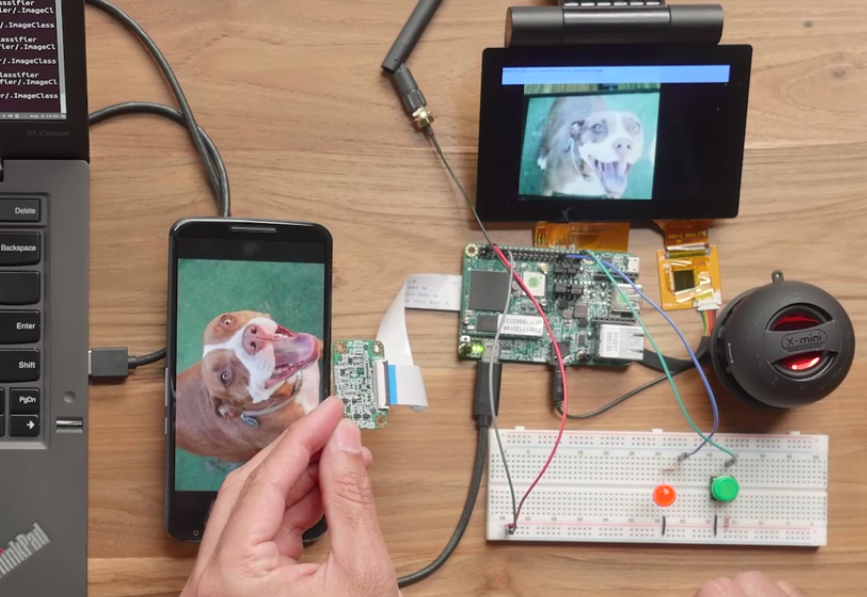
\includegraphics{hardware}}  
		\centering
		\caption{Hardware Model}
		\label{fig:hardware}
		\end{figure}

		\subsection{Android Things} \label{subsection:android}

		A resource efficient and feature-rich operating system, Android Things, was chosen as the base for the software required for this project. Android Things extends the core Android framework with additional APIs provided by the Things Support Library, which lets us integrate with new types of hardware. In-built libraries and APIs help provide the most efficient solutions to common hardware interfacing situations.\\
		\newline
		There are provisions for regular Over-The-Air (OTA) security updates and software patches by building on top of the Android OS. This allows the device to be updated remotely and with the latest OS. The Pico i.MX7D used for this project was flashed with Android 8.1 (Oreo) with the latest April 2018 security patch.

		\begin{figure}[h] 
			\centering
			\resizebox{8cm}{4cm}{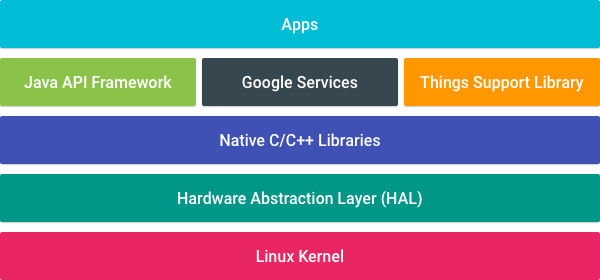
\includegraphics{android}}  
			\centering
			\caption{Android Things Framework}
			\label{fig:android}
			\end{figure}

	\subsection{Tensorflow Lite Setup} \label{subsection:tensorflow}

	TensorFlow Lite is TensorFlow’s lightweight solution for mobile and embedded devices. It enables on-device machine learning inference with low latency and a small binary size. TensorFlow Lite also supports hardware acceleration with the Android Neural Networks API.\\
			\newline
	TensorFlow Lite uses many techniques for achieving low latency such as optimizing the kernels for mobile apps, pre-fused activations, and quantized kernels that allow smaller and faster (fixed-point math) models.\\
	\newline
	Code:
	\begin{verbatim}
private void doRecognize(Bitmap image) {

// Allocate space for the inference results
byte[][] confidencePerLabel = new byte[1]
[mLabels.size()];

// Allocate buffer for image pixels.
int[] intValues = new int
[TF_INPUT_IMAGE_WIDTH*
TF_INPUT_IMAGE_HEIGHT];

ByteBuffer imgData=ByteBuffer
.allocateDirect(
DIM_BATCH_SIZE * TF_INPUT_IMAGE_WIDTH 
* TF_INPUT_IMAGE_HEIGHT * DIM_PIXEL_SIZE);

imgData.order(ByteOrder.nativeOrder());

// Read image data into buffer formatted
// for the TensorFlow model
TensorFlowHelper.
convertBitmapToByteBuffer(image, intValues
, imgData);

// Run inference on the network with 
the image bytes in imgData as input,
// storing results on the 
// confidencePerLabel array.
mTensorFlowLite.run
(imgData, confidencePerLabel);

// Get the results with the highest 
//confidence, map them to their labels
Collection<Recognition> results = 
TensorFlowHelper.getBestResults
(confidencePerLabel, mLabels);
// Report the results with the 
//highest confidence
//onPhotoRecognitionReady(results);
}

	\end{verbatim}

\subsection{Classification} \label{Classification}

Google Tensorflow researchers developed a lightweight neural network model called MobileNet and published pre-trained versions of it for image recognition, trained with a bit more than one million images from ImageNet classified within 1000 categories (or "classes", in machine learning parlance).

In the initClassifier() method, we read this model and the labels associated with each of the 1000 categories (like "dishwasher", "Border collie" or "English springer").

In the doRecognize() method, the code extracts the pixels of the given image in a way compatible to how the network was trained: 24 bits per pixel of the original image, one for each basic color (red, green and blue). Also, the image is required to have 224x224 pixels, so the image is resized if necessary.

Once the pixels stored on imgData buffer in a format that is compatible with the inputs expected by the neural network, we run the inference that classifies the image — this is where the actual magic happens. The network is massive, and running it involves a lot of numeric computation. This step itself takes around half second on a Raspberry Pi 3.

The results from running the network are returned as an array of float confidence levels ranging from 0 to 1 per category. A higher value means a stronger confidence that the photo is of that category. The getBestResults() method in the TensorFlowHelper class finds the highest values and returns their labels.

	\section{Future Work} \label{section:conclusion}

		The Image Classifier is a feasible solution to assist specially-abled people in perceiving and interacting with the world in a better way. It offers a cost-effective solution using embedded devices and efficient on-board Machine Learning algorithms to perform its classification actions.\\
	  The prototype be improved in certain ways such as:
	
	\begin{enumerate}
	\item Use of higher quality camera: Increasing camera quality will allow there to be a greater degree of accuracy in identifying the model.
	\item More powerful compute devices and integration with mobile phones. The use of Android Things allows us flexibility in offloading compute processes to a more powerful mobile device that the user may possess.
	\item Use of a Vibration Motor to accentuate warnings of fast approaching objects such as vehicles.
	\item Converting the prototype to a full functioning product: Once the prototype is tested for all possible test cases, it must be made into a finished product. For that, the software architecture should be resilient for several conditions like poor lighting, fast movement, horizontal scan, etc. Extensive testing will be required and other hardware solutions should be considered and iterated upon.
	\end{enumerate} 
	
	\begin{thebibliography}{9}
		\bibitem{Cortex-M4} 
		
		\textit{Cortex-M4 Technical Reference Manual}. 
		ARM, 1993.
		\\\texttt{https://developer.arm.com/docs/100166/0001}
		 
		\bibitem{Pico} 
		Pico i.MX7D 
		\textit{Datasheet}. 
		NXP, 2017.
		\\\texttt{https://www.nxp.com/docs/en/data-sheet/IMX7DCEC.pdf}

		\bibitem{Tensorflow} 
		Tensorflow Lite
		\textit{}. 
		Google, 2018.
		\\\texttt{https://www.tensorflow.org/mobile/tflite/}
		\end{thebibliography}
	
	\end{document}
	
	